\documentclass[11pt]{article}
\usepackage[a4paper, top=4cm, bottom=3cm, left=3cm, right=3cm]{geometry}
\usepackage{geometry} % see geometry.pdf on how to lay out the page. There's lots.
\geometry{a4paper} % or letter or a5paper or ... etc
% \geometry{landscape} % rotated page geometry
\usepackage[english]{babel}
%\usepackage[utf8]{inputenc}
%\usepackage{accents}
\usepackage{graphicx}
\usepackage{array}
\usepackage{multirow}
%\usepackage{mathptmx}
%\usepackage{amsmath}
%\usepackage{makeidx}
\usepackage{verbatim}
\usepackage{amssymb}
\usepackage{latexsym}
\usepackage{comment}
\usepackage{sectsty}
\usepackage{accents}
\usepackage{natbib}
\usepackage{caption}
% See the ``Article customise'' template for come common customisations
\newcolumntype{x}[1]{{\centering\hspace{0pt}}p{#1}}

% By Simon ==================================================


\newcommand{\simon}[1]{\vspace{1em}(\emph{Simon: #1})\vspace{1em}}

%TIKZ====
\usepackage{tikz}
\usetikzlibrary{arrows,shadows,petri,positioning}
%\usetikzlibrary{fit}					% fitting shapes to coordinates

% End by Simon =============================================


\title{ICT for Basic Service Delivery - Case Study: Water Sector in Uganda}
\author{
\small{Ikae Catherine Omal}\\
\small{School of Computing and Informatics Technology, University of Makerere, Uganda}\\ \small{\textit{ikae.catherine@cit.mak.ac.ug}}\\
}

\date{\today}

\begin{document}
\maketitle

\begin{abstract}

\end{abstract}



%%%%%%%%%%%%%%%%%%%%%%%%%%%%%%%%%%%
%Introduction
\section{Main objectives and research hypotheses}\label{objectives}
The main objective will be to understand how mobile phone services can be improved and adjusted to the combined context of developing countries (Uganda) and crowdsourced monitoring (water maps) to ensure improved access to water. Our main assumption is that up-to-date and accurate information is crucial for the correct allocation of resources and budget dedicated to water infrastructures. This is the also the assumption shared by many new water mapping projects in Africa\footnote{Rural Water Supply Network (RWSN): http://www.rural-water-supply.net/en/}. Such a research is therefore especially crucial at a time when more and more institutions (governments and NGOs) are relying on end-user provisions of infrastructure information to allocate new investments and to ensure general quality of services. For example, new ``crowd-­maps"\footnote{Crowd maps allow anybody to provide geo-­based information (e.g. reports, reviews, or pictures) on topics that are important for them and for front providers and governments.} have been set up to capture the status of important infrastructure (Ushahidi, NextDrop, H20initiative), requested actions for failing infrastructure (Huduma) or crucial news in times of conflicts or disasters (Libya Crisis Map, Geofeedia), with varying degrees of success. 
\\
In the typical African context of largely scattered rural populations, the ability to use sms-based monitoring on services access can greatly reduce monitoring costs and misallocations, a priority for budget-constrained governments. It promises also better governance through greater transparency and increased participation from end-users. According to the World Bank (2004), ``successful services for poor people emerge from institutional relationships in which the actors are accountable to each other". Shared information and communication could therefore be an attractive solution to foster these mutual accountabilities. 
\\\\
However, while the benefits of mobile-based, user-centric information seem clear, the level of participation across communities remain very low, both in terms of external intensity (the number of people using the mobile reporting tools) and internal intensity (the number of messages sent back to the central entity). Without the full participation of end-users, most ICT projects are destined to fail, which represents a massive opportunity loss. Our assumption is that most of this problem is due to an  inadequacy between the mobile services and their targeted demographic, in terms of ease of use (language, interface), incentives (absence of feedbacks and recompense for the effort) and social dynamics (target the individuals in a community-driven context). When a system is simple to use and has clear value (such as m-payment MPESA), uptake and usage rates are much higher. We aim to attain a same level of participation for the provision of information destined to populate water maps.  
\\\\
To succesfully achieve this goal, the proposed research will form a sequence of 4 different research ``modules":
\begin{enumerate}
\item
We will analyze the current context in our target research field: who are the people using phones; what are the current ICT (mostly phones) penetration, usages and types (simple or smartphone); what are the biggest barriers to usage (complexity, lack of perceived rewards, technical hurdles); what are the forms and frequency of mobile communications (sms, voice...); what is the recognized value of monitoring and reporting on water infrastructure.
\item
We will experiment with the designs of the communication channels/ user-interfaces (UI) used to provide the bottom-up information on water: nature of the message (SMS, email, voice…), language used (multi-lingual, symbol-based), actions required (forms, dialed-in choice selection, special number-to-action, voice messengers…). In general, choices about design will be informed by the results of the context analysis. For instance, it is probable that we start our experimentations with SMS, knowing that SMS is highly popular in Uganda due to their limited costs and ubiquity\footnote{According to the Ugandan Communications Commission, 294 million SMS messages were sent during the January–March 2009 period, compared to 190 million in the preceding quarter (October–December 2008).}.
Each interface will then be tested in a randomized experiment to assess its effectiveness on the amount of data sent back (data density) and to account for the influence of external drivers (education, gender, wealth...)
\item
Following the experimental pattern of the previous module, we further experiment with the implementation of feedbacks and rewards messages to inform the end-users about the value of water reporting. 
This aspect is especially important since we expect the lack of feedbacks to be one of the key drivers of low participation levels across many water mapping projects.
We also plan to integrate network-centric rewards such as community checks (e.g. cross-validation of messages) or possible gamification tools (e.g. points-to-purchase scheme) to improve internal intensity. 
\item
Finally and using the collected information, we will test for the nature of the data sent back (data quality), in terms of content and degree of details. Modules of pattern recognition (via machine-learning) will be implemented to categorize and classify data and to assess the influence communication channels and feedback schemes have on the quality of information collected (while accounting for socio-economic characteristics). This aspect should give us insights generalizable to other sectors and functions.
\end{enumerate}  
The thesis will benefit from a close integration with a larger multi-disciplinary project on ``mobile ICT for public services under weak public institutions" under the joint-supervision of Ass. Prof.Isabel G\"{u}nther (ETH NADEL) and Prof.Gerhard Tr\"{o}ster (ETH Electronic Labs) and with the active collaboration of several research insitutes in Switzerland and in sub-Saharan Africa (ETH-­NADEL, ETH-­SOMS, ETH-­Electronics Lab for Switzerland, Makerere School of Computing and IT for Uganda, iHub Research for Kenya, and University of Dar es Salaam for Tanzania). In particular, the field part of the thesis will be coordinated with Prof.Florence Tushabe at the School of Computing and IT at Makerere University (Uganda). The water-related aspects will benefit from close interactions with Dr. Richard Johnston from EAWAG (Zurich) and from Dr. Niwagaba from the Civil and Environmental Engineering Department at Makerere University.  

\section{Field context}
\subsection{Targeted region}
For the implementation of this proposed doctoral thesis, we target the Ugandan district of Wakiso, which has a total area of 2,704 km$^{2}$ and an estimated total population of 1,310,100. It is made up of two counties: Kyaddondo County and Busiro County. 
\\
Considering that the district cannot be covered in its entirety due to time and budget constraints, the proposed field target is the Kakiri Municipality, which lies approximately 17 kilometers northeast of the central business district of the city of Kampala, the Uganda's capital. This town presents multiple advantages for the success of this project: it is close to the capital, with an important and easily accessible population and with a evenly distributed gender population (48.5\% of men for 52.2\% of women, according to \citep{population2010} and \citep{population02}). Across the other key characteristics of interest (wealth, education, type of employment, source of revenues, water access), the municipality spans a large variety of education, activity and wealth profiles. It is also at the junction of urban and rural districts, which will allow for some analysis of potential urban/rural discrepancies. Moreover and quite importantly, water access there is a collective and difficult process, the object of frequent tensions among the population. It is therefore an excellent field for assessing new ICT tools targeting water management and provision.
\subsection{The ICT context}
Based on a rapid field survey in the Kakiri municipality, it appears that most people are embracing mobile phone technologies and using them on a daily basis, not only to access but also to share information freely. In general, mobile phones have become basic needs to many Ugandans because people rely on them to access a wide range of services: from market prices to mobile Banking (mMoney) to Mobile Health (mHealth).
Moreover, mobile phones are used more and more for data collection and dissemination across multiple sectors, such as health, socio-economic development, agriculture, natural resource management, disaster relief, and their relevant sub-sectors. In health, mobile phones are employed to disseminate information on public health to residents and health workers and to manage inventories of drugs in remote locations among other things. In agriculture, mobile phones connect farmers to government services, cooperatives, and networks, as well as facilitate the flow of timely information about markets and crop prices. Mobile banking, or mBanking, has made financial services more attractive and readily accessible to poor populations and those living in remote locations\cite{Rikke10}. Mobile phones hold particular value in these fields because they can act as point-of-use devices, function in remote locations, and are readily carried and used at any time \cite{Kimberly11}\cite{Rikke10}.
\\
However, ICT penetration and the multiplication of new services in urban and well-off areas of Uganda should not mask a diversity of context among Ugandan regions. Studies have revealed that rural inhabitants and poorer urban users value phone services but do not use them very often compared to relatively more affluent users; over 40\% of people in Uganda used mobile phones through friends and family and individuals; although a further 24\% of people used mobile phone through teleshops, demonstrating a strong preference for mobile phones rather than landlines, and a preference for private phones rather than public access points. It has also been shown that ``chatting" with friends and family is clearly the most common use of phones in Uganda\cite{ Scott04}. Overall, Uganda has moved from approximately 250,000 available fixed telephone lines pre-2003 to over 17 million available mobile lines by the second quarter of 2012 and a penetration of more than 50\% (16.45 million mobile phone subscribers), thereby making Ugandan telecommunications market one of the fastest growing in Africa\footnote{The main telecom operators in Uganda are MTN, Airtel, UTL, Warid and Orange Uganda.}. According to PWC, this penetration rate should expand to 70\% by 2015 (25 million users) 
\\
ICT now drives some activities in the financial and tourism and informal sectors while various e-Government initiatives are ongoing in various departments at all tiers of government\cite{Nora10}\cite{Post11}. 
\\\\
However, numerous barriers to mobile phone usage remain in Uganda. The primary obstacle is the lack of comprehensive communication infrastructure across the country (especially in rural areas), which manifest itself through unreliable and expensive electric supply, limited network access and prohibitive communication costs. To alleviate these challenges in our project, we hope to benefit from the results of another Sawiris scholar on opportunistic communications (Abdullah Alhussainy, ETH CSG), whose network choices may provide an alternative in remote and disconnected areas. The second obstacle is the limited mobile proficiency of the end-users, a barrier we will rightfully address through our research project (by improving design and limiting cognitive effort). 

\subsection{The state of user-based ICT in Uganda}
An important success factor for our project is the degree of awareness of the population on the potential of ICT for used-based actions (crowdsourcing). If end-users are aware that mobile phones can be used to report and share information with positive results, it can only improve the interest of local people for our research and experiments. Fortunately, ICT tools have been used on several occasions in Uganda and information provision is slowly becoming mainstream.
\\
For instance, ICT tools were used to empower people to participate in the democratic processes of the February 2011 presidential elections\cite{Post11}, providing alternative mediums of communication and engagement and allowing citizens to express views that might otherwise not have been tolerated if they were to voice them through mainstream media\cite{Post11}\cite{ Ashnah12}. ICT also served to monitor the elections with two initiatives, Uchaguzi\footnote{Uchaguzi, run by the Citizens Coalition for Electoral Democracy in Uganda (CCEDU) and other civil society organizations, aggregated ``citizens" and election observers' voices in near real time on the elections, incorporating mobile phones, mapping tools, twitter and Facebook on its online portal\cite{Post11}.} and Uganda Watch 2011, allowed to report the political events as they happened. Combined with other tools such as SMS short codes, online forms, email and Twitter, the platforms helped to achieve fair and transparent elections in real-time\cite{Post11}\cite{ Ashnah12}.
While most of these experiments are still young, they demonstrate that Uganda considers ICT tools as means to empower end-users and improve governance. We are therefore confident of the feasibility of our project in this context.


\section{State of research in the field}\label{state_of_research}
Should cover state of research and references (point3), and innovativeness of research/ research methodology (point4) + corresponding logical framework (whatever that is)

\simon{To Do}

\begin{itemize}
 \item jana formerly txteagle
 \item FrontlineSMS
 \item RapidSMS
 \item ushahidi
 \item h20initiative
 \item rwsn.ch
 \item m4water.org
 \item waterpointmapper.org
\end{itemize}


\section{Methodology}\label{methodology}
\subsection{Methodology}\label{metho}
Should give in full details the methodology to be used (point4)
\begin{figure}
\begin{center}
 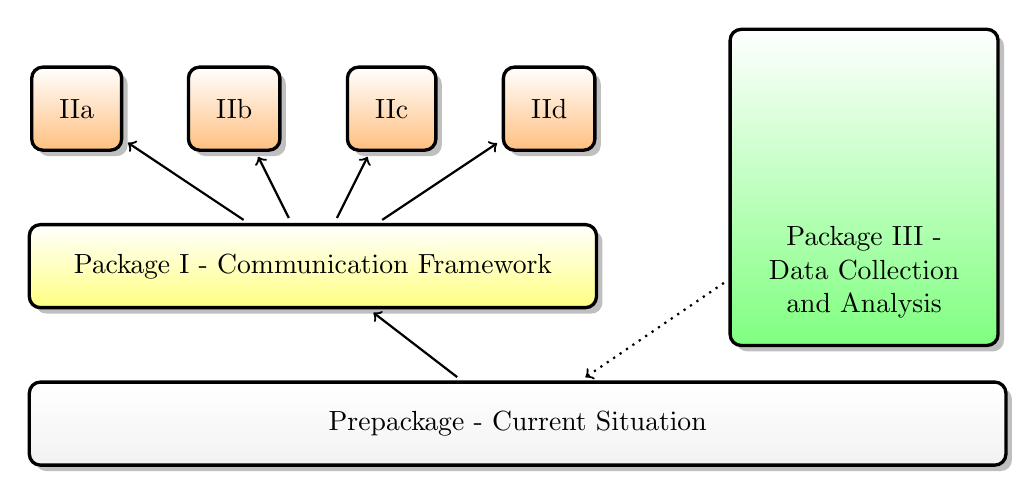
\begin{tikzpicture}[node distance=1.5cm, shorten >=2pt, shorten <=2pt, thick, auto]


\tikzstyle{box} = [
    rectangle,rounded corners,draw=black, top color=white, very thick, inner sep=1em, minimum size=3em,drop shadow]

 
\node[box, bottom color=gray!10, text width = 11.7cm, text centered] at (-1.4,0) (prepackage) {Prepackage - Current Situation};

\node[box, bottom color=yellow!50, text width = 6.5cm, text centered] at (-4,2) (packagei) {Package I - Communication Framework};

\node[box, bottom color=green!50,  text width = 2.7cm, text height = 2.4cm, text centered] at (3,3) (packageiii) {Package III - Data Collection and Analysis};


\node[box,  bottom color=orange!50] at (-7,4) (packageiia) {IIa};

\node[box,  bottom color=orange!50] at (-5,4) (packageiib) {IIb};

\node[box,  bottom color=orange!50] at (-3,4) (packageiic) {IIc};

\node[box,  bottom color=orange!50] at (-1,4) (packageiid) {IId};



\path[->]
  (prepackage) edge (packagei)
  (packagei) edge (packageiia)
  (packagei) edge (packageiib)
  (packagei) edge (packageiic)
  (packagei) edge (packageiid)
;

\path[->, dotted]
  (packageiii) edge (prepackage)
;


\end{tikzpicture} 
\end{center}
\caption{Research packages hirarchy}
\label{tikz:researchpackages}
\end{figure} 
\citet{champanis2012reporting} state: \begin{quote}
``Based on our experience and focus on rural environments, our
approach to ICT development has been that the investigation of
the local context and solutions responding to local needs are more
valuable and sustainable than a general “one-size-fits-all” design.
Whilst this speaks against the notions of “scalability”, which is
usually a desired outcome for IT solutions, we believe that rural
and under-resourced environments require a more detailed and
customised solution.''\end{quote} 

A set of research packages is presented that allows to build up a well tailored but still scalable solution that - beside of helping people directly -  gives space to investigate on research relevant questions in the field of computer science and further sociology, development aid and economics. 

Figure~\ref{tikz:researchpackages} explains the research packages hierarchy: The small Prepackage analyses the context. In Package I the main framework for future project plug-ins is designed. The actual scientific part from a computer science perspective is done in Package II whose subpackages can be implemented individually. Package III is a parallel ongoing process that profits from improvements in Packages I\&II.


\subsubsection*{Package I: Analysis of the current situation}
\paragraph{Goal} Get an overview of mobile ICT usage and water management in rural Uganda
\paragraph{Method}
In the field of mobile ICT information is aggregate from cooperation with governmental institutions, local service provides and by detailed literature study:
\begin{enumerate}
 \item Distribution of cell phones (by model, user age, area)
 \item Usage distribution (by time, frequency and service)
 \item Analysis of finances (income per user, cost of different services per user, money spent for different services per user)
 \item Analysis of technology (cellular network standards, cell sizes, user per cells, quality of service, future investments, availability of electricity)
 \item Analysis of hindrances for a more frequent usage (finances, easy of use, illiteracy, privacy concerns)
\end{enumerate}
In the field of drinking water additional input comes from partnership with local NGOs.
\begin{enumerate}
 \item Analysis of the drinking water need amongst population and its challenges
 \item Further data will be collected during the project as a result of Package III
\end{enumerate}


\subsubsection*{Package II: Design of a communication channel}
\paragraph{Goal} Design a inter-user communication channel that is user friendly, low-cost, reliable, secure and information rich
\paragraph{Method} A first substep evaluates different communication channels. Text-, graphical- and voice based methods are compared on different generations of phones. Depending on their connection standards (GSM, GPRS, 3G) and application platforms supported (SMS, Java Me, Android) best possible options are chosen. Challenges occur in the following areas:
\begin{itemize}
 \item Low cost feature phones (``a modern low-end mobile phone that is not a smart phone'' [Wikipedia]) are widely available in Uganda. Their drawback is that software has to be implemented manufacturer depending and in general allows just limited functionality \cite{champanis2012reporting}.
 \item Access to provider data (calls with user id, text messages, cell info) is difficult to obtain. A possible solution is to use just mobile data services and transfer messages based on an extra developed service.
 \item Literacy rate of Uganda is around 66 percent [Wikipedia]. Tailored solutions for illiterates have successfully been implemented \cite{brown2012water}. By developing special input methods, one has to be aware that a very important reason for people to buy a phone is due to its associated status and not its features \cite{knoche2012text}.
 \item Low cost transmission is necessary to achieve a high user participation. Prices for SMS make up a higher percentage of the monthly budget than in high income countries. An alternative approach is to provide hardware and airtime to selected user group in order to conduct studies.
 \item Free hardware and airtime is likely to be misused. Champanis and Rivet report that ``Users would fill up the phone with music and video downloads'' \cite{champanis2012reporting} to an extend that it is not usable for the experiment anymore.
 \item User trust and information security is one of Africas biggest challeng, this due to weak privacy laws, user awareness, political instability and not maintained software \cite{goodman2010coming}.
\end{itemize}

In a second substep we analyse the information flow needed to provide a water quality information and monitoring network. The implementation (third substep) completes Package I. To the moment it remains an open question if a self designed device for data transmission over the mobile network would fulfil this purpose even better than a cell phone based service. 

The success of such an system is unpredictable. Hence we suggest an iterative approach based on trial and error method. Lessons learned from other projects are considered and results reported to the community.



\subsubsection*{Package IIIa: Quality control}
\paragraph{Goal} Achieve high quality information collected at a centralised agent but also sent to individual receivers 
\paragraph{Method} According to \cite{birnbaum2012automated} supervised and unsupervised machine learning methods are feasible to classify manually generated data in health surveys in Tanzania and Uganda. Widely used machine learning algorithms could be modified in order to not just classify but rather rate user message according to a scale of trust. Additionally the knowledge of the crowd is used to label messages and hence a  supervised learning on initially unlabelled data is performed - similar to a supervised spam filter. Out of this, a general trust giving and learning (human and machine based) distributed network could be generated.

This contains the following areas of risk:

\begin{itemize}
 \item The reported lack of data quality in surveys in low income countries could also be the result of the normally used top-down approach \cite{birnbaum2012automated}, whereas a bottom-up approach  (where users have a personal interest on the quality of the data) might not even, or at least less face this problem.
 \item The question resides if a machine learning solution for such a difficult task is an actual benefit for a country where human workforce is cheap (and jobs needed) and technology expensive. We would not be surprised if a mixed solution - highlighting suspicious messages machine- and final classification human based - might be the best solution.
\end{itemize}

\subsubsection*{Package IIIb: Context analysis}
\paragraph{Goal} Gather context data of users and messages and provide information accordingly

\paragraph{Method}
Four different fields of study can be divided:
\begin{description}
 \item [User context] Albeit low cost feature phones provide just limited sensor functionality, they allow nevertheless access to basic context information like position (Cell site or GPS), time and number of contacts (address book). Out of this, additional contextual information like weather condition can be added.
 \item [Message content and context] To get a meaningful information transfer on water quality between humans and a machine it is mandatory to understand the content of a message either by the use specific questioning and answer mechanisms (e.g. input form) or by mining data out of unspecific messages. Later is current field of research, e.g in the area of text messages \cite{aggarwal2012mining}. This gives a high degree of freedom to test, redesign and evaluate state of the art algorithms. Once functioning methods are available, they can be used as well to support subfield one (User context) by mining additionally user context information out of the exchanged messages. 
 \item [Context information provision] Having filtered data, most relevant information is provided to the users, (e.g. closest working water source, closest available mechanic, water shortage in specific area, water preparation information). The task is either done by a machine- or human agent for which a specific interface would be designed.
 \item [Contextual information presentation] The gained context information can be used to present the information in more readable way, e.g. by using specific graphics.
\end{description}

Risks in this package are low since goals and functionality are scalable depending on success of basic experiences.

\subsubsection*{Package IIIc: Water mapping}
\paragraph{Goal} Map water status information on the web
\paragraph{Method} Together with local partners\footnote{http://wwww.spactialcollective.com} an interface is designed that allows spacial mapping on a web platform.

\subsubsection*{Package III: Incentives and gamification}
\paragraph{Goal} Analyze incentive methods to get more user participation, by strengthening the link between user contribution and rewards, using both the \emph{intrinsic motivation} for the mobile scheme (gamification) and the \emph{extrinsic motivation} coming from network externalities (transparency, peer pressure).
\paragraph{Method}
Insights collected with Packages I and IIb will be used to create different form of social incentives that we will apply to our intelligent network design. We will first experiment with persuasive technologies \citep{Oinas_Kukkonen2010, fogg2002persuasive} and internal gamification techniques \citep{blaschkeextrinsic, crowley2012gamification} to assess their performance to increase water reporting in our sample. Our assumption, which is in line with the literature, is that the intrinsic motivation of gamification can elicit internal motivation that ensure re-engagement and continuous participation \citep{lin2008elucidating, ling2005using}. It is also proven that its effects are improved in presence of network externalities \citep{lin2011people}. We will then test for extrinsic motivators (rewards, feedbacks on usefulness) and compare the performance of the two groups of incentives. We will structure our research using recent research on motivation theory \citep{davis1992extrinsic, kim2007value}
\paragraph{Risk}
The main risk lies in our ability to implement network-based extrinsic motivations. If we are unable to map networks appropriately, we may have to limit our research to intrinsic motivators such as pure gamifications, rewards and feedbacks. 


\subsubsection*{Package IV: Data collection and analysis}
\paragraph{Goal} Use the built system to collect data and use it for further improvements
\paragraph{Method}

\begin{itemize}
 \item If successful, the platform from Project I and the modules from Project II provide a large amount of data that can be used even outside the scope of the water sector and computer science. Since data is accumulated from the first implementation of Project I, this is a parallel ongoing process.
 \item The interface to a centralized human agent (introduced Package IIb) can be used to conduct surveys where the data accumulated from the bottom-up network does not provide the necessary information.
 
 \item Information collected on water access (average distance traveled for water access, pump durability, water well users profile) can be used to improve Package I\&II.
\end{itemize}

\section{Organization}\label{organization}
As already mentioned, the thesis will benefit from its close relation to a larger multi-disciplinary project on ``mobile ICT for public services under weak public institutions" under the joint-supervision of Ass. Prof.Isabel G\"{u}nther (ETH NADEL) and Prof.Gerhard Tr\"{o}ster (ETH Electronic Labs), with the active collaboration of several research institutes in Switzerland and in sub-Saharan Africa (ETH-­NADEL, ETH-­SOMS, ETH-­Electronics Lab for Switzerland, Makerere School of Computing and IT for Uganda, iHub Research for Kenya, and University of Dar es Salaam for Tanzania).  
\\
The candidate will work on the field with several NGOs and companies that specialize in mobile application and services for an African audience. On SMS communication, she will supported by the team of Frontline SMS, the leader in SMS campaign communication. She will also benefit from discussions and results from other teams in Tanzania and Kenya, such as Ushahidi and its iHub research lab\footnote{http://www.ihub.co.ke/pages/home.php} in Kenya and Twaweza in Tanzania\footnote{http://twaweza.org/}.
\\\\
The analyze of the current context will be a main responsibility of the PhD candidate, benefiting from her own personal field and the cumulative experience of Frontline SMS, Ushahidi, Twaweza and Prof.Tushabe. It should ensure a proper understanding of the ICT idiosyncrasies in the Ugandan context.
\\
Design templating for the mobile interfaces will be performed in conjunction with the ETH Electronics Labs and the water sector specialists (EAWAG and the Civil and Environmental Engineering Department at Makerere University). The design, conduct and analysis of the different field experiments will be supervized by the economic team at ETH NADEL.
\\
Feedbacks and reward mechanisms, relying heavily on individual and collective sociology, will be approached and validated in coordination with the social scientists at ETH SOMS.
\\
Finally, the data content analysis will benefit from the help of the NADEL team (for statistical methodologies), the Electronic Labs engineers (from the design of the machine learning filters) and the partners in Uganda (Makerere University) who will help contextualize the results.    
\\\\
As a future PhD candidate, Catherine Ikae Omal, who has a background in Computer Sciences, will be under the direct supervision of Prof.Tr\"{o}ster at the Electronic Labs while extensively working with the other departments and institutes involved. In particular, her field work will be assisted by Prof.Florence Tushabe for the Computer Science components. Prof.Isabel G\"{u}nther will also provide extensive guidance in the design and coordination of the different field experiments.
\\\\
While we are confident that the project is structured to avoid the major pitfalls, important uncertainties remain around the uptake of this project in its targeted local communities. There is a risk that the project falls prey to the same disaffection affecting current mobile projects on water reporting. To mitigate this risk, a first backstop will be the completion of the first module of research. By providing an extensive and up-to-date analysis of the existing usage of ICT in Uganda, this project will provide important context to better understand the lack of participation in mobile schemes. This corresponds for us to the worst-case scenario.
\\
Under a less negative hypothesis, our research will manage to develop and test several new communication channels and to assess their performance. We plan to openly share our findings and open-source our models, which will ensure a certain amount of traction among researchers and operational actors. Therefore, even in the unlikely case where randomized experiments are impossible to implement, we are confident that the project will still greatly improve mobile services for water access.


\section{Expected results}\label{expected}
\subsection{Expected results}
We expect to improve both the understanding of the drivers behind mobile reporting (at least for the water sector) and the nature of the mobile services (apps) and schemes to be develop to ensure high participation rates from end-users. A first block of results will be research-based, with new insights on the hurdles, usages and means of improvements for ICT in the Ugandan context. While many projects invoke mobile communications as a new tool to reduce poverty, very few scientific evidence have been gathered so far on mobile capacities and challenges to increase monitoring, governance and resource allocation. 
\\
A second block of result will be the creation of several tested communications schemes to improve end-user participations. To our knowledge, this will be the first time that context, feedbacks, incentives and network influence will be properly and scientifically addressed in the design of mobile apps. There is therefore a large potential for improvement of mobile services based on the results of this project and for replication of our findings. Its potential reach is reinforced by our tight integration with the key players in this field (Frontline SMS, Ushahidi) who will assure large dissemination of our findings in Africa.
\subsection{Strategy for their implementation}
This project intends to have a significant impact on both researchers and policy makers. Communication to the research community about our results will follow the traditional path of producing working papers, submitting articles to peer-­reviewed journals and attending conferences. Our implementation strategy will first come from the tight partnership with influential actors in the mobile ICT and crowdsourcing field from the beginning of the research project (Ushahidi, Twaweza, Frontline SMS). This partnership will lead to a number of open-­source mobile applications and internet platforms and full-­‐scale examples of implementations on which future projects can be based. Last, we plan to write a couple of short policy briefs to be distributed among interested agencies, and to organize at least two specific policy workshops for interested governments, NGOs and bi-­ and multilateral development agencies to discuss the benefits and challenges of mobile ICT for water monitoring and reporting. Given that the project works within the water sector and with mobile technologies, the potential for replication in other countries will be large: over a billion people are still without access to improved water, and mobile technologies have shown tremendous growth rates with three quarter of the planet’s population having access to mobile phones in varied social, cultural and economic contexts.

\section{Budget}

Detailed budget for each year of the scholarship, differentiating all funding sources including those of the ETH chair and partner contributions (financial or in-kind) (point10) -> Jonathan


\bibliographystyle{model2-names}
\bibliography{Sawiris2013}


\end{document}